\chapter{Systèmes linéaires invariants}
\label{chap:lti}
Le but de ce chapitre est de présenter les concepts de base
indispensables à l'étude des systèmes linéaires à temps invariants
LTI\footnote{ Linear Time Invariant} et des signaux.  Après une
définition des critères qui caractérisent un système LTI, nous
chercherons à répondre à la question suivante : comment déterminer
efficacement la réponse d'un système linéaire lorsqu'il est soumis à
une excitation quelconque ?  Par efficacement, nous entendons :
\begin{itemize}
\item méthode mathématiquement "simple"~;
\item méthode indépendante de l'excitation et des propriétés du
  système LTI.
\end{itemize}


Pour cela, nous commencerons par nous interroger sur la manière de
représenter l'interaction entre l'entrée et la sortie d'un système,
puis sur les notions d'excitation et de réponse. Nous distinguerons
les notions de réponses naturelles et forcées, avant d'identifier deux
familles d'excitation adaptées à l'étude des systèmes : exponentielle
complexe et impulsionnelle. Nous introduirons ensuite la notion de
fréquence (complexe), qui nous offrira la possibilité d'étudier les
signaux temporels dans le domaine fréquentiel, ainsi que la notion de
fonction de transfert qui facilitera l'étude des systèmes.
	
	
\section{Définition d'un système linéaire invariant}

	\subsection{Linéarité} 
	Un système relie à chaque signal d'entrée $x$ un signal de
        sortie unique $y$. Les signaux $x$ et $y$ sont des fonctions
        de la variables réelle appartenant à un espace de fonction le
        plus général possible noté ici $L_E$. La relation
        entrée-sortie est donc modélisée par une application
        mathématique de $L_E$ dans $L_E$ notée $L$ et définie ainsi~:
	\begin{equation}
          L : \application{L_E}{L_E}{x : t\mapsto x(t)}{y : t\mapsto y(t)} 
          % DONE : correction TYPAGE et remarque notation
	\end{equation}

	\begin{remarque}{}
          Remarquons que l'application $L$ transforme une fonction en
          une fonction et que cela peut compliquer les notations,
          aussi il est courant de voir utiliser les crochets [] autour
          des fonctions arguments de l'application $L$ et les simples
          parenthèses autour de la variable réelle argument d'une
          fonction. Ce genre d'application est souvent désignée par le
          terme d'\emph{opérateur}
	    
          Beaucoup d'abus de notation figurent dans la littérature,
          gardons à l'esprit et tentons cette année encore de
          conserver une rigueur d'écriture irréprochable pour garder
          les idées claires. Parmi les écritures suivantes, une est
          parfaitement correcte et représente un réel~; une représente
          correctement une fontion mais ne respecte pas la convention
          des crochets~; une est incorrecte~; une est correcte mais
          lourde à écrire. À vous de les retrouver~:
          \begin{itemize}
          \item $y(t) = L[x(t)]$~;
          \item $y = L(x)$~;
          \item $y(t) = L[x](t)$~;
          \item $t\mapsto y(t) = L[t\mapsto x(t)]$
          \end{itemize}{}
	\end{remarque}
	
	Une classe de système fondamentale est la classe des systèmes
        linéaires car elle offre de nombreux outils et propriétés
        mathématiques.
	\begin{definition}{Système linéaire}
          \label{def:linearite}
          
          Une système est dit linéaire si et seulement si
          l'application $L$ associée est linéaire, soit pour tout
          $\p{x_1,x_2,\lambda} \in L_E^2 \times \R$~:
          \begin{eqnarray}
            \label{eq:def_linearite}
	    \forall t \in \R \qquad L\b{x_1 + \lambda\, x_2}(t) = L\b{x_1}(t) + \lambda\,L\b{y_2}(t) \nonumber\\
	    \text{ou bien } \qquad L\b{x_1 + \lambda\,x_2} = L\b{x_1} +\lambda L\b{x_2 }
          \end{eqnarray}
	\end{definition}
	

	Une des conséquences de la linéarité est la possibilité
        d'appliquer le principe de superposition.
	
	% TODO on va considérer d'autres systèmes ! j'enlèverai cette
	% partie qui n'amène pas grand chose...
	Les trois opérateurs linéaires de base que nous considérons
        dans l'étude des systèmes linéaires sont :
	\begin{itemize}
        \item proportionnel : $y = a x$ où a est une constante
        \item intégration : $y = a \int f(x) \deriv x $ où a est
          une constante
        \item dérivée : $y = a \frac{df(x)}{dx} $ où a est une
          constante
	\end{itemize}
	On peut aisément vérifier qu'il respecte la condition
        \ref{eq:def_linearite}.
	% Fin du dodo

        \begin{remarque}
          Pour résoudre les complexes équations différentielles des
          télégraphistes, \Heaviside{} utilise ces opérateurs de base
          et introduit le \emph{calcul symbolique}. Cela consiste à
          représenter l'application de l'opérateur dérivée sur une
          fonction $f$ comme une simple multiplication par un nombre
          $p$. Ainsi une équation différentielle
          $a\,y'' + 2y' -y = 3\int x$ est associée à l'équation
          symbolique $a\,p^2\,y + 2\,p\,y - y = \frac{3}{p}x$. Il est
          alors possible de résoudre algébriquement l'équation sous
          forme de fractions rationnelles ce qui donnerait avec notre
          exemple~: $y = \frac{3/p}{a\,p^2+2p+1} x$. Rappelons que $x$
          et $y$ sont des fonctions et non des réels et que dans ce
          cas les opérations ne sont pas de simple multiplication et
          addition de réels mais bien des multiplications et additions
          de fonctions. La variable symbolique $p$ est utilisée comme
          un nombre réel mais n'est en aucun cas un réel...
        \end{remarque}
	
	\subsection{Invariance temporelle}
	% DONE rédaction en définition
	Il est fréquent qu'un système réagisse de la même manière
        indépendemment de l'instant où est appliqué le signal
        d'entrée. Ce qui conduit à la définition suivante~:
	\begin{definition}{Système invariant dans le temps}
          
          Un système est dit invariant dans le temps si et seulement
          si son application associée $L$ vérifie~:
          \begin{equation}
            \forall x\in L_E, \forall (t,t_0)\in \R^2, \quads L[t\mapsto x(t-t_{0})] = L[x](t-t_{0}) 
          \end{equation}
	\end{definition}
	
	En d'autres termes, la réponse du système ne dépend pas de
        l'origine des temps choisie.
        
	\begin{exemple}
          % TODODONE typage !!!
          L'effet d'un système sur le signal d'entrée est d'écrit par
          l'application ~: $x \mapsto y=2\dDtDe{x}$.  Vérifions
          d'abord que cet opérateur est linéaire~:
          \begin{eqnarray*}
            L\b{x_1+\lambda x_2} &= t \mapsto 2\, \dDt\p{x_1+\lambda x_2}\\
                                 &= t \mapsto 2\,\dDtDe{x_{1}} + 2\lambda\,\dDtDe{x_{2}}\\
                                 &= L\b{x_{1}}+\lambda\,L\p{x_{2}}
          \end{eqnarray*}
          Le système est donc linéaire. Vérifions qu'il est
          invariant~:
          \begin{equation*}
            \forall t \quads L\b{t\mapsto x(t-t_{0})}(t) =2\,\dDe{x\p{t-t_0}}{\p{t-t_0}}\,.\,\underbrace{\dDe{\p{t-t_0}}{t}}_{=1}=2\dDtDe{x}\p{t-t_0}=L\b{x}\p{t-t_0}
          \end{equation*}
          ou bien exprimé par le biais des opérateurs en exprimant le
          retard d'un temps $t_0$ par le biais de l'application
          identité soit $\Id-t_0 : t \mapsto t - t_0$ ~:
          \begin{equation*}
            L\b{t\mapsto x(t-t_{0})} = L\b{x \circ \p{\Id-t_0}}=2\,\dDt\p{x\circ\p{\Id -t_{0}}}=2\,\dDtDe{x}\circ\p{\Id-t_0}\,.\,\underbrace{\dDt\de{\Id-t_0}}_{=1}=L\b{x}\circ\p{\Id-t_0}
          \end{equation*}
        \end{exemple}
	
        % TODODONE pas d'accord là ! Un simple gain de 2 est un
        % système qui n'est pas passif...
        % à discuter
        %	\subsection{Passivité}
        %	Dans ce cours, on considèrera aussi des systèmes
        % passifs, dans le sens où il n'y a pas d'énergie emmagasinée
        % ou fournie par une entrée autre que celle sur laquelle on
        % applique le signal d'entrée étudié.
      
	\subsection{Causalité}
	L'étude des systèmes linéaires passent par l'étude et la
        synthèse de fonctions mathématiques. Tous les systèmes
        linéaires physiquement réalisables peuvent être décrits par
        une fonction mathématique linéaire. Par contre, la réciproque
        n'est pas forcément vraie : un système décrit par une fonction
        linéaire n'est pas nécessairement physiquement réalisable. Une
        caractéristique importante qui différencie les systèmes
        physiquement réalisables de ceux qui ne le sont pas est la
        notion de causalité. On entend par physiquement réalisable un
        système pouvant traiter en temps réel les signaux d'entrée.
        Dans un système causal, l'effet ne peut pas précéder la cause,
        ce qui donne la définition suivante.
        \begin{definition}{Système causal}
          \label{def:causal}
          
          Un système est causal si, et seulement si, la propriété suivante est vérifiée pour tout $t_0 \in\R$~:
          \begin{equation}
            \label{eq:def_causal}
          \forall t<t_{0} ,\;  x(t) = 0 \quads\implies\quads \forall t<t_{0},\; y(t) = 0
	\end{equation}   
        \end{definition}

       	Les systèmes numériques peuvent être non causaux car ils sont
        capables de stocker les valeurs du signal d'entrée pour un
        traitement différé. On peut prendre l'exemple de l'application
        de floutage d'une image numérique. Celle-ci correspond à une
        matrice de données, représentant chaque pixel de l'image. Le
        floutage consiste à appliquer un filtre (par exemple gaussien)
        qui sera centré sur chaque pixel. Ce filtre effectue une somme
        pondérée du pixel central mais aussi des pixels voisins,
        situés avant et après le pixel central. L'effet du floutage
        d'un pixel dépend donc de pixels situés après dans l'ordre de
        rangement des pixels.

	
	
	\section{Equation générale d'un système linéaire}
        Un système linéaire invariant est gouverné par une équation
        différentielle à coefficient constant donnée dans sa forme
        générale par \ref{eq:generale_lti}. On l'appelle l'équation
        générale du système. Pour une excitation $x(t)$ donnée, sa
        résolution permettra de déterminer la réponse $y(t)$.	
	\begin{eqnarray}\label{eq:generale_lti}
          L : x \mapsto y \text{ telle que }\quads &\sum_{n=0}^N{a_{n}\,\dDtDeOrdre{y}{n}} = \sum_{m=0}^M b_{m}\, \dDtDeOrdre{x}{m}\\\nonumber
       \iff & a_0\,y + a_1\,\dDtDe{y} +\ldots + a_{N}\,\dDtDeOrdre{y}{N} = b_0\,x + b_1\,\dDtDe{x} +\ldots + b_{M}\,\dDtDeOrdre{x}{M} 
        \end{eqnarray}
	
	
	\section{Réponse d'un système}
	La réponse d'un système correspond au signal (ou aux signaux)
        de sortie lorsqu'il est excité par un (ou plusieurs) signal
        d'entrée. En reprenant l'équation générale
        \ref{eq:generale_lti}, on remarque que l'on peut
        distinguer :
	\begin{itemize}
        \item une réponse propre ou naturelle d'un système, notée
          $y_{H}(t)$, correspondant à une solution de l'équation
          différentielle homogène~: \cad{} pour une excitation nulle.
        \item la réponse forcée, notée $y_{f}(t)$ correspondant à la
          solution particulière de l'équation différentielle associée
          à une excitation particulière $x(t)$.
	\end{itemize}
	
	La réponse naturelle $y_h$ appartient à un espace des
        solutions homogènes noté $S_H$ et sera déterminée en fonction
        des conditions initiales. La réponse d'un système sera la
        superposition de ces deux réponses.
	\begin{equation}
          y(t) = \underbrace{y_{H}(t)}_{\in S_H} + y_{f}(t)          
	\end{equation}
	
	Dans la suite du cours, nous ne nous intéresserons qu'à des
        systèmes causaux, et nous considérerons, sans perte de
        généralité, que les excitations sont nulles pour $t < 0$.
	
	\section{Réponse naturelle d'un système LTI}
	Il s'agit de la partie de la réponse qui est indépendante de
        l'excitation, \cad{} la solution de l'équation homogène. Elle
        est donc intrinsèque aux caractéristiques du système. Elle se
        détermine en résolvant l'équation différentielle
        \ref{eq:generale_lti} dans le cas où l'excitation $x(t)$ est
        nulle.
	\begin{equation}\label{eq:reponse_naturelle}
          \sum_{n=0}^N a_{n}\, \dDtDeOrdre{y}{n} = 0
	\end{equation}

        % %%TODO petite erreur, je parlerai des conditions initiales ici
	% On pourrait s'interroger sur le sens de cette réponse. Si le
        % système n'avait pas emmagasiné d'énergie au départ, la réponse
        % serait nulle, ce qui ne présente pas d'intérêt pour l'étude
        % des systèmes. La réponse naturelle n'apparait que si le
        % système a été préalablement excité avant t = 0.
        % DONE je propose
        \begin{remarque}
          On peut s'interroger sur le sens physique de la recherche
          d'une solution non--nulle pour $t>0$ alors que le système
          n'est pas excité (un second membre nul correspondant à une
          entrée nulle). L'intuition physique nous laisse penser
          qu'une réponse non nulle n'apparaîtrait que si le système a
          été préalablement excité avant ou pendant $t = 0$, puis \og
          relâché \fg{} par une excitation nulle pour tout $t>0$.

          Lorsque l'on ne souhaite pas s'intéresser à ce qui précède
          l'instant $t_0=0$ et à ce qui a pu amener le système dans un
          état d'excitation (énergie emmagasinée dans les composants
          etc.), on considère alors une excitation et une réponse
          nulle pour tout $t<t_0$ et on ajoute des conditions
          initiales non nulles à l'instant $t_0$ représentant l'état
          du système (tensions et courant initiaux dans un système
          électrique par exemple) avant le lâché à l'instant $t_0$.
      \end{remarque}

        
        % %%TODO ben non ! elle apparait à t>0... peut être parler
        % %% des manières d'ammener un système à son état initial...
	% Comme l'excitation disparait pour t > 0, la réponse sera
        % forcément transitoire. Seule une fonction présentant la même
        % forme avant/après dérivation plusieurs fois peut être solution
        % de l'équation \ref{eq:reponse_naturelle}. Il n'existe
        % qu'une seule forme de fonction avec une telle propriété : la
        % forme exponentielle complexe donnée par (\ref{expo_complexe}).

        %% TODO le faire en annexe 
        %%TODO et si on disait qu'on s'intéresse aux solutions de formes
        %% exponentielle : on le justifie par l'expérience et en math par
        %% par un passage de l'équadiff à une forme matricielle compagne.
        % DONE je propose

      Rappelons que pour les équations différentielles d'ordre 1,
      l'espace des solutions homogènes est généré par toute
      combinaison linéaire d'une seule solution
      $y_0$ de forme exponentielle réelle~:
      \begin{equation}
        \label{eq:sol_homogene_ordre_1}
        S_H=\a{\lambda y_0|\lambda\in\R}=\vect{y_0},\quads \text{avec } L\b{y_0}=\nullDe{L_E},\quads \text{et } y_0: t\mapsto \expo{\alpha\,t},\;\alpha \in \R 
      \end{equation}

      Dans le cas d'équations d'ordre supérieur, la recherche de
      solutions de forme exponentielle non nulles
      $t\mapsto \expo{p\,t}$ vérifiant l'équation homogène donne en
      remplaçant dans \eqref{eq:reponse_naturelle}~:
      \begin{eqnarray} \label{solution_reponse_naturelle} \forall
        t\in\R,\quads \sum\limits_{n=0}^N a_{n}\,\dDtDeOrdre{\expo{p
            t}}{n} =
        \sum\limits_{n=0}^N a_{n}\,p^{n} \expo{p\,t} =\underbrace{\expo{p\,t}}_{\neq 0}\;\sum\limits_{n=0}^N a_{n}\,p^{n}  =0\\
        \implies D(p)= \sum_{n=0}^N a_{n} p^{n} = 0
      \end{eqnarray}

      Le polynôme $D(p)$ est appelée l'équation caractéristique du
      système d'équations différentielles. Pour un système d'ordre
      $N$, ce polynôme est scindé dans $\C$ et possède donc $N$
      racines réelles ou complexes conjuguées telle que
      $D(p)=a_N\,\prod\limits_{i=1}^{N-1}\p{p-p_i}$. Ces racines sont appelées
      pôles du système et notées $p_i$ (i de $1$ à $N$). Les
      caractéristiques de la réponse naturelle du système sont liées
      uniquement aux $N$ solutions, ou pôles $p_{i}$, de cette
      équation.

      % La réponse naturelle peut alors s'écrire sous la forme suivante~:
	% \begin{equation}\label{reponse_naturelle}
        %   y_{H}(t) = \sum_{i=1}^N A_{i} \expo{p_i\,t}
	% \end{equation}
	% où les termes $A_{i}$ dépendent des conditions initiales
        % connues en un temps $t_{0}$.	
	% Ce polynôme est appelée l'équation caractéristique du
        % système. En effet, les caractéristiques de la réponse
        % naturelle du système sont liées aux M solutions ou racines
        % $p_{i}$ de cette équation. La réponse naturelle peut alors
        % s'écrire sous la forme suivante :
	% \begin{equation}\label{reponse_naturelle}
        %   y_{0}(t) = \sum_{i=1}^M A_{i} \expo{p_i\,t}
	% \end{equation}
	% où les termes $A_{i}$ dépendent des conditions initiales
        % connues en un temps $t_{0}$.	
        
      On montre que les solutions homogènes des équations
      différentielles d'ordre $N$ à coefficients constants sont des
      combinaisons linéaires de $N$ exponentielles $y_i$ à
      coefficients réels et/ou paire de complexes conjuguées. L'espace
      des solutions homogènes est donc un espace de dimension $N$
      généré par la famille $\a{y_i}_{i=1\dots N}$ de $N$
      exponentielles complexes~:
	\begin{equation}\label{eq:sol_homogene_ordre_n}
          S_H=\vect{\a{y_i}_{i=1\dots N}},\quads \text{avec } L\b{y_i}=\nullDe{L_E}\quads\text{et }y_i : t\mapsto \expo{p_i\,t},\quads p_i\in\C     
	\end{equation}

        La réponse naturelle peut alors s'écrire sous la forme
        suivante~:
	\begin{equation}\label{eq:reponse_naturelle}
          \forall t\in\R,\quads y_{H}(t) = \sum_{i=1}^N \lambda_{i} \expo{p_i\,t}
	\end{equation}
	où les termes $\lambda_{i}$ dépendent des conditions initiales
        connues en un temps $t_{0}$.	
        
	\subsection{Fréquences naturelles d'un système LTI}
	Les $N$ racines de l'équation caractéristique du systèmes sont
        appelées les fréquences naturelles ou fréquences propres du
        système. Elles sont complexes et de la forme suivante :
	\begin{equation}\label{freq_propre}
          p_{i} = \sigma_{i} + j\omega_{i} 
	\end{equation}	
	En reprenant \ref{eq:reponse_naturelle}, la réponse naturelle
        pourra s'exprimer en fonction de ces fréquences naturelles :		
	\begin{equation}\label{eq:reponse_naturelle_freq}
          y_{0}(t) = \sum_{i=1}^M \lambda_{i}\expo{\sigma_{i}t}\,\expo{j\omega_{i}t}
	\end{equation}
	$\omega_{i}$ caractérise la pulsation de la réponse associée à
        cette racine, tandis que la partie réelle $\sigma_{i}$ indique
        l'atténuation ou l'amortissement de cette réponse. Leur
        connaissance est indispensable car ce sont elles qui
        caractérisent la forme temporelle de la réponse du système. La
        prédiction de l'évolution temporelle de la réponse du système
        va passer par l'analyse de ces racines.
	
	\subsection{Plan de \Laplace}
	Puisque les racines de l'équation caractéristique déterminent
        la réponse naturelle d'un système, il est intéressant
        d'établir un système de représentation graphique facilitant
        l'analyse du système. C'est le but de la représentation
        appelée plan complexe, plan de \Laplace{} ou plan P, illustré
        à la figure \ref{Fig:Plan_P}. Il s'agit d'un repère cartésien
        dans lequel les racines sont placées, permettant de visualiser
        leurs parties réelles et imaginaires. Selon le positionnement
        des racines dans le plan complexe, les caractéristiques du système
        seront différentes, notamment sa stabilité.
	\begin{figure}[htbp]
          \centering 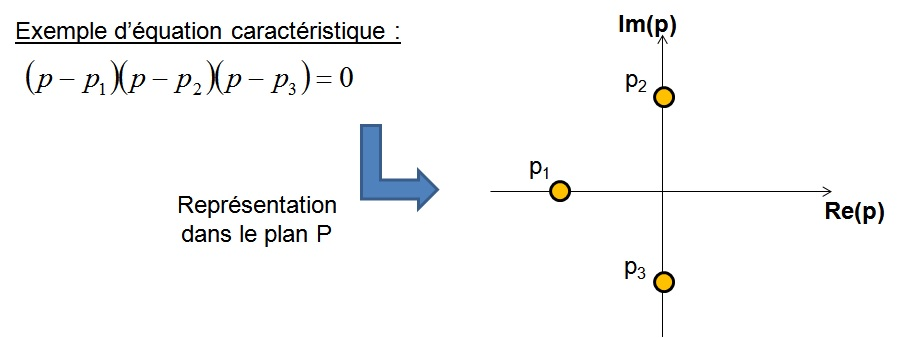
\includegraphics[scale=0.5]{images/Plan_P.jpg}
          \caption{Placement des racines de l'équation caractéristique
            dans le plan complexe. La racine $p_1$ est réelle
            négative~: apportant une exponentielle décroissante à la
            réponse. Tandis que $p_2$ et $p_3$ sont purement complexes
            conjuguées et apportent deux exponentielles complexes
            conjuguées, et donc par la formule d'\Euler{} une forme
            sinusoïdale pure, à la réponse.}
          \label{Fig:Plan_P}
	\end{figure}

	% \subsection{Analyse du plan complexe - Stabilité du système}
        % %%TODO def de strabilite fausse
	% La stabilité d'un système est une notion qui sera abordée plus
        % en détail dans les cours d'automatique. Dans ce cours, nous
        % utiliserons une définition au sens large : on entend par
        % stabilité le fait que la réponse d'un système converge vers
        % une valeur finie quelle que soit l'excitation appliquée (à
        % condition que cette excitation converge). Dès que l'on conçoit
        % un système, c'est une propriété indispensable qui doit être
        % vérifiée.  Un système est stable si et seulement si à toute
        % entrée bornée, il fait correspondre une sortie bornée :
        % DONE je preprend en proposant

        La stabilité d'un système est une notion qui sera abordée plus
        en détail dans les cours d'automatique, il s'agit en fait
        d'une propriété intrinsèque du système ne dépendant pas de
        l'excitation. Dans ce cours, nous utiliserons une définition
        au sens large~: on entend par stabilité le fait que la réponse
        naturelle ne diverge pas. Dès que l'on conçoit un système,
        c'est une propriété indispensable qui doit être vérifiée.

        \begin{definition}{stabilité d'un système}
          \label{def:stabilite}
          
          Un système est stable si, et seulement si, à toute entrée
          bornée, il fait correspondre une sortie bornée~:
	\begin{equation}
          \exists A\in\R,\;\forall t \in \mathbb{R},\quads \abs{x(t)} \leq A \quads\implies\quads \exists B\in\R,\; \forall t\in\R,\quads \abs{y(t)} \leq B
	\end{equation}
        \end{definition}

        Dans le cas des systèmes LTI, cette définition est équivalent
        à la définition suivante~: un système est stable si toute
        réponse naturelle tends vers 0 à l'infini. Dans ce cas là la
        notion de stabilité est clairement indépendante du type
        d'excitation.

        La position des racines de l'équation caractéristique
        détermine à la fois la stabilité du système linéaire, mais
        aussi la forme temporelle de réponse.

        La figure ci-dessous illustre les types de réponse naturelles
        associées à une fréquence naturelle, selon sa position dans le
        plan complexe.
	\begin{figure}[htbp]
          \centering
          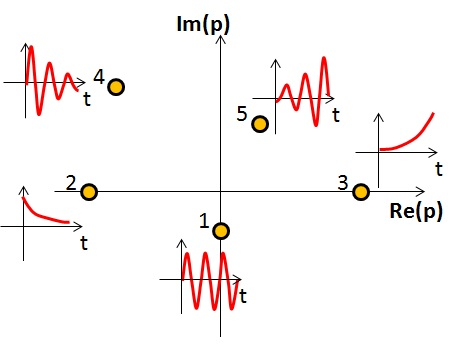
\includegraphics[scale=0.5]{images/reponse_vs_p.jpg}
          \caption{Types de réponse naturelle en fonction de la
            position d'une racine dans le plan complexe.}
          \label{Fig:reponse_vs_p}
	\end{figure}
        Considérons les cinq cas suivants, correspondant à cinq
        positions différentes d'une racine $p_{i}$ dans le plan
        complexe, et déterminons le type de réponse temporelle. On
        considère t > 0 :
	\begin{enumerate}
        \item $p_{i}$ est purement complexe ($\sigma_{i}$ = 0) : elle
          est située sur l'axe des ordonnées du plan complexe. La réponse
          naturelle sera donc un signal purement (co)sinusoïdale, dont
          l'oscillation aura une fréquence ou une pulsation déterminée
          par $\omega_{i}$. Le système est en limite de stabilité car
          sa réponse oscille en permanence autour d'une valeur.
        \item $p_{i}$ est purement réel et négatif ($ \sigma_i\leq 0$
          et $ \omega_i = 0$)~: la racine est située sur l'axe des
          abscisses à gauche de l'origine. La réponse est une fonction
          exponentielle décroissante, sans la moindre oscillation,
          indiquant un comportement amorti. Le système est stable
          asymptotique.
        \item $p_{i}$ est purement réel et positif ($ \sigma_i\geq 0$
          et $ \omega_i = 0$)~: la racine est située sur l'axe des
          abscisses à droite de l'origine. La réponse est une fonction
          exponentielle croissante, sans la moindre oscillation,
          indiquant un comportement divergeant. La réponse naturelle
          indique un système instable.
        \item $p_{i}$ est une valeur complexe quelconque dont la
          partie réelle est négative ($ \sigma_i< 0$ et
          $\sigma_{i} \neq 0 $) : la racine est située dans le demi
          plan à gauche de l'axe des ordonnées. La réponse va
          présenter une oscillation dont la fréquence est déterminée
          par $ \omega_{i}$, mais dont l'amplitude s'atténue
          exponentiellement plus ou moins rapidement au cours du temps
          selon la valeur $\sigma_{i}$. Cette réponse indique un
          système stable oscillatoire amortis.
        \item $p_{i}$ est une valeur complexe quelconque dont la
          partie réelle est positive ($\sigma_i > 0$ et
          $ \omega_{i} \neq 0 $) : la racine est située dans le demi
          plan à droite de l'axe des ordonnées. La réponse va présenter
          une oscillation dont la fréquence est déterminée par
          $ \omega_{i} $, mais dans l'amplitude s'accroît exponentiellement plus ou
          moins rapidement au cours du temps selon la valeur
          $\sigma_{i}$. Cette réponse indique un système oscillatoire instable.
	\end{enumerate}

        % %TODO comprend pas trop l'objectif final... me parait dangereux...
	% \textbf{\underline{Domaine fréquentiel}}	
	% On remarque que l'on est capable de représenter avec un point
        % dans le plan p une fonction temporelle de type exponentielle
        % complexe. Il s'agit de la même fonction, mais vue dans un
        % autre domaine, que l'on appelle domaine fréquentiel. Dans ce
        % domaine, la fonction n'est plus caractérisée par le temps,
        % mais par sa fréquence. De manière générale, les fréquences
        % sont des grandeurs complexes. Néanmoins, dans le cas de
        % l'analyse des signaux, on ne considère que des fréquences
        % réelles.
	
	
	\subsection{Ordre d'un système linéaire}
	Plus l'équation caractéristique présente de racines, plus sa
        réponse devient complexe, puisqu'elle résulte de la
        superposition de plusieurs fréquences comme le montre
        l'équation \ref{eq:reponse_naturelle}. On appelle l'ordre d'un
        système le nombre de racines que présente son équation
        caractéristique. Il s'agit aussi de l'ordre ou du degré de
        l'équation différentielle caractérisant le système. Pour
        illustrer la notion d'ordre, nous allons analyser la réponse
        naturelle de deux circuits électriques passifs, caractérisés
        par des équations caractéristiques d'ordre 1 et 2. Vous
        retrouverez une analyse plus détaillée dans le cours
        d'électronique.
	
        \begin{exemple}{circuit RC}
          \label{ex:circuit_rc}
          
          \begin{minipage}[l]{0.7\linewidth}
            On considère le circuit ci-contre, formé par une résistance
            R et un condensateur C. En t = 0, le condensateur est
            chargé, de sorte que la tension à ses bornes soit égale à
            $U_{C0}$. On note $U_{C}$ et $U_{R}$ les tensions aux bornes
            du condensateur et de la résistance.
          \end{minipage} \hfill
          \begin{minipage}[r]{0.4\linewidth}
            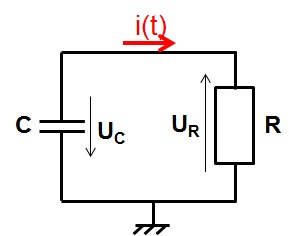
\includegraphics[scale=0.5]{images/circuit_RC_reponse_naturelle.jpg}
          \end{minipage}
          
          On souhaite déterminer la réponse naturelle de ce circuit pour
          $t > 0$, sous la forme du courant électrique $i(t)$ circulant au
          travers du circuit. On souhaite aussi déterminer la fréquence
          naturelle de ce circuit, caractérisant sa réponse transitoire.
          
          
          Commençons par appliquer la loi des mailles à ce circuit, qui
          permet d'écrire : $U_{R}(t)+U_{C}(t)=0.$ En prenant en compte
          les relations tension-courant pour la résistance et le
          condensateur, cette relation peut être mise sous la forme
          ci-dessous ne faisant apparaître que le courant. Après
          différenciation de l'équation, on fait apparaître une équation
          différentielle du premier ordre. On constate que le terme RC
          est homogène à un temps. On l'appelle la constante de temps du
          circuit RC, généralement notée $\tau$.
          \begin{equation*}
            R\,i(t)+\frac{1}{C}\int i(t) \deriv t=0~\implies ~\dDtDe{i}(t)+\frac{1}{RC}\,i(t) = 0
          \end{equation*}
          On retrouve une équation du même type que
          \ref{eq:reponse_naturelle}. La solution de cette
          équation peut donc s'écrire : $i(t) = A\expo{pt}$, où A est lié
          aux conditions initiales et p est l'unique fréquence naturelle
          du système. En intégrant cette solution dans l'équation
          différentielle, on en déduit l'équation caractéristique de ce
          circuit (\ref{equa_carac_RC}).
          \begin{eqnarray*}
            \label{equa_carac_RC}
            \forall t\in\R,\quads A\,p\,\expo{pt}+\frac{1}{RC} \expo{pt}=0 \nonumber\\
            \iff p+\frac{1}{RC}=0 \iff p-\underbrace{\frac{-1}{RC}}_{p_{0}}=0
          \end{eqnarray*}
          Cette équation présente une seule racine $p_{0} =
          -\frac{1}{RC}$. Ce circuit électrique est donc un système
          d'ordre 1. La racine est purement réelle et négative. Elle se
          situe donc à gauche de l'axe des imaginaires dans le plan complexe,
          traduisant le comportement stable et non oscillant du système
          (équivalent au point 2 de la figure
          \ref{Fig:reponse_vs_p}). La fréquence naturelle indique donc
          une réponse naturelle du type exponentielle décroissante. Cela
          est confirmé par l'expression de la réponse naturelle du
          circuit, qui s'écrit :
          \begin{equation}\label{Reponse_naturelle_RC}
            i(t)=A\expo{p_{0}t}=A\expo{-\frac{t}{RC}},\quads \forall t>0
          \end{equation}
          La valeur de A peut être déterminée à partir des conditions
          initiales en t = $0^{+}$. Le courant dans le circuit est alors
          donné par : $i(0)=\frac{U_{R}(0)}{R}=\frac{U_{C0}}{R}$. A
          partir de \ref{Reponse_naturelle_RC}, on en déduit
          $A=\frac{U_{C0}}{R}$.
        \end{exemple}
        
        \begin{exemple}{circuit RLC}
          \label{ex:circuit_rlc}
          
          \begin{minipage}[l]{0.7\linewidth}
            On considère le circuit ci-contre, formé par une résistance
            R, un condensateur C et une bobine L montées en parallèle
            (R, L et C $\geq$ 0). En $t= 0$, le condensateur est chargé,
            de sorte que la tension à ses bornes soit égale à
            $U_{C0}$. On note $i_{C}$, $i_{R}$ et $i_{L}$ les courants
            traversant ces trois composants.
          \end{minipage} \hfill
          \begin{minipage}[r]{0.4\linewidth}
            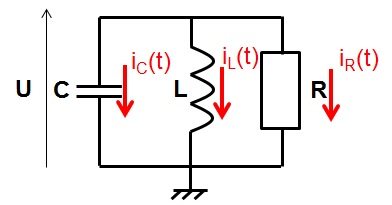
\includegraphics[scale=0.5]{images/circuit_RLC_reponse_naturelle.jpg}
          \end{minipage}
          
          On souhaite déterminer la réponse naturelle de ce circuit pour
          $t > 0$, sous la forme de la tension $u(t)$ mesurée aux bornes du
          circuit. On souhaite aussi déterminer la fréquence naturelle
          de ce circuit, caractérisant sa réponse transitoire.
          
          
          Commençons par appliquer la loi des
          nœuds à ce circuit, qui permet d'écrire :
          $i_{C}(t)+i_{R}(t)+i_{L}(t)=0$. En prenant en compte les
          relations tension-courant pour la résistance et le
          condensateur, cette relation peut être mise sous la forme
          ci-dessous, ne faisant apparaître que le courant. Après
          différenciation de l'équation, on fait apparaître une équation
          différentielle du second ordre. Pour simplifier les notations,
          on pose : $\alpha = \frac{1}{2RC} $ et
          $\omega^{2} = \frac{1}{LC}$.
          \begin{eqnarray*}
            C\dDtDe{u}+\frac{u(t)}{R}+\frac{1}{L}\int u(t) \deriv t=0 \quads\implies\quads \dDtDeOrdre{u}{2}+\frac{1}{RC}\dDtDe{u}+\frac{1}{LC}\,u(t) = 0\\
            \dDtDeOrdre{u}{2} + 2\alpha \dDtDe{u}+\omega^{2}u(t) = 0
          \end{eqnarray*}
          
          On retrouve une équation du même type que
          \ref{eq:reponse_naturelle}. Un vecteur solution de cette
          équation peut donc s'écrire : $u(t) = A\,\expo{pt}$. En intégrant
          cette solution dans l'équation différentielle, on en déduit
          l'équation caractéristique de ce circuit~:
          \begin{eqnarray}
            \label{eq:carac_RLC}
            \forall t\in\R\quads \p{p^{2}+2\alpha p+\omega^{2}}A\expo{pt}=0 \nonumber\\
            \iff  p^{2}+2\alpha p+\omega^{2}=(p-p_{1})(p-p_{2})=0
          \end{eqnarray}
          Cette équation présente deux racines $p_{1}$ et $p_{2}$. Ce
          circuit électrique est donc un système d'ordre 2, dont la
          réponse naturelle va s'écrire :
          \begin{equation}\label{key}
            u(t) = A_{1}\expo{p_{1}t}+A_{2}\expo{p_{2}t}
          \end{equation}
          
          où $A_{1}$ et $A_{2}$ dépendent des conditions
          initiales. Selon la valeur de R, L et C, la nature et la
          position de ces racines dans le plan complexe va changer, modifiant
          le comportement transitoire du circuit. Pour déterminer ces
          racines, il suffit de résoudre une équation d'ordre 2, dont le
          déterminant est donné par :
          $\Delta = 4(\alpha^{2}-\omega^{2})$. La nature des racines
          varie selon le signe du déterminant :
          \begin{equation}
            si~\alpha \geq \omega : \left \{
              \begin{array}{l}
                p_{1}=\frac{-2\alpha +\sqrt{\Delta}}{2}=-\alpha+\sqrt{\alpha^{2}-\omega^{2}} \\
                p_{2}=\frac{-2\alpha -\sqrt{\Delta}}{2}=-\alpha-\sqrt{\alpha^{2}-\omega^{2}} \\
              \end{array}
            \right.
          \end{equation}
          \begin{equation}
            si~\alpha < \omega : \left \{
              \begin{array}{l}
                p_{1}=\frac{-2\alpha +j\sqrt{-\Delta}}{2}=-\alpha+j\sqrt{\omega^{2}-\alpha^{2}} \\
                p_{2}=\frac{-2\alpha -j\sqrt{-\Delta}}{2}=-\alpha-j\sqrt{\omega^{2}-\alpha^{2}} \\
              \end{array}
          \right.
	\end{equation}
	On peut distinguer plusieurs types de comportement transitoire
        distincts selon les valeurs de $\alpha=\frac{1}{2RC}\geq 0$ et $\omega=\frac{1}{\sqrt{LC}\geq 0}$~:
	\begin{itemize}
        \item si $\alpha \neq 0$, alors les deux racines présentent
          une partie réelle négative. Le système présente donc un
          caractère stable.
        \item si $\alpha \geq \omega$, les deux racines sont purement
          réelles et négatives. Dans le plan complexe, elles sont situées sur
          l'axe des réels à gauche de l'axe des imaginaires. La
          réponse du circuit sera du type exponentiel décroissant sans
          oscillation (équivalent au point 2 de la figure
          \ref{Fig:reponse_vs_p}).
        \item si $\alpha < \omega$ et $\alpha \neq 0$, les deux
          racines sont conjuguées. Elles sont situées à gauche de
          l'axe des imaginaires dans le plan complexe. La réponse du circuit
          sera du type oscillation amortie de pulsation
          $\sqrt{\omega^{2}-\alpha^{2}}$ (équivalent au point 4 de la
          figure \ref{Fig:reponse_vs_p}).
        \item si $\alpha = 0$, les deux racines sont purement
          imaginaires et conjuguées. Elles sont placées sur l'axe
          imaginaire du plan complexe, symétriquement à l'axe de réels. La
          réponse du circuit sera une oscillation non amortie de
          pulsation $\omega$ (équivalent au point 1 de la figure
          \ref{Fig:reponse_vs_p}).  Cela correspond au cas 
           $R=0, C\neq 0$ d'une résistance nulle
          entretenant des oscillations perpétuelles (stabilité limite
          ou simple)
	\end{itemize}
      \end{exemple}
	
	\section{Réponse forcée}
	
	La réponse forcée est la solution de l'équation générale du
        système pour une excitation non nulle. La réponse va dépendre
        de la forme de l'excitation, mais aussi des propriétés du
        système. Puisque la réponse dépend de l'excitation, il est
        préférable de déterminer des excitations dont les propriétés
        faciliteront l'analyse de la réponse forcée d'un système. Pour
        cela, il faut chercher des familles d'excitation dont la forme
        n'est pas modifiée par l'effet du système LTI. Ainsi, en
        connaissant la forme de l'excitation, on déduira immédiatement
        la forme de la réponse. Seuls quelques coefficients que nous
        préciserons seront à calculer.
	
	Nous allons nous intéresser à deux familles d'excitations
        répondant à ce critère : l'excitation exponentielle complexe
        (que nous avons rencontré précédemment) et la famille
        d'excitation impulsionnelle.
	
	\subsection{Excitation exponentielle complexe}
	L'excitation exponentielle complexe présente la forme suivante~:
	\begin{equation}\label{eq:exc_expo_complexe}
          x =    \left \{
            \begin{array}{l l}
              \hat{X}  \expo{p_{x}t}  & si~t>0 \\
              0   & sinon \\
            \end{array}
          \right .
	\end{equation}
	
	où $ \hat{X} = |x| \expo{j \theta}$ est l'amplitude complexe,
        ou vecteur de Fresnel, ou le phaseur du signal. Et
        $p_{x} = \alpha +j\,\omega $ sa fréquence complexe. Dans le
        cas où l'on s'intéresse à des signaux réels (cas rencontré en
        pratique), cette forme reste valable à condition de ne
        conserver que la partie réelle. Elle s'écrit alors :
	\begin{equation}\label{eq:exc_expo_complexe_reel}
          x(t) =    \left \{
            \begin{array}{l l}
              \Reel{\hat{X}  \expo{p_{x}t}} = |X|  \expo{\alpha t}  cos(\omega t+\theta)  & si~t>0 \\
              0   & sinon \\
            \end{array}
          \right .
	\end{equation}
	Comme dans le cas de la fréquence naturelle, la fréquence
        complexe peut être représentée dans le plan complexe. Sa position
        indique qualitativement la forme temporelle de
        l'excitation. Si p\textsubscript{x} est purement réelle,
        l'excitation est une fonction exponentielle pure. Si
        p\textsubscript{x} est purement imaginaire, l'excitation est
        une fonction cosinusïdale pure. L'excitation est dite
        monochromatique. |X| représente son amplitude et $\theta$ sa
        phase.
	
        \begin{exemple} Récrivez les expressions des fonctions
          ci-dessous sous la forme de fonctions réelles :
          $y(t)=Re[(1+j)\expo{(-2+j)t}]$ et
          $z(t) = Re[2\expo{j\frac{\pi}{2}}\expo{j10t}]$.Les deux
          fonctions sont des exponentielles complexes. Elles
          représentent des signaux temporels réels puisqu'on ne
          conserve que la partie réelle.

          Le phaseur de la fonction
          $y(t)$ peut s'écrire
          $\hat{Y}=1+j=\sqrt{2}\expo{j\frac{\pi}{4}}$. La fréquence
          complexe est $p_y=-2+j$. Elle contient une partie réelle
          négative donnant un comportement d'exponentielle
          décroissante de constante de temps $2$ à l'amplitude, et une
          partie imaginaire donnant un comportement oscillant de
          pulsation égale à $1$. La fonction $y(t)$ peut donc s'écrire~:
          \[y(t)={\sqrt{2}}\expo{-2t}cos(t+\frac{\pi}{4})\]

          En procédant de même pour la fonction $z(t)$, on remarque
          que sa fréquence est purement complexe de pulsation 10, son
          phaseur est d'amplitude $2$ et de phase $\frac{\pi}{2}$. Il
          s'agit d'une fonction cosinusoïdale s'écrivant :
          $z(t)=2\,cos(10\,t+\frac{\pi}{2})$.
      \end{exemple}
	
	
      L'excitation exponentielle complexe a une propriété remarquable
      : l'action d'un opérateur linéaire (proportionnel, intégrateur
      ou différentiel) laisse sa forme inchangée. Seule son amplitude
      complexe (phaseur) sont modifiées. On peut donc en déduire une
      propriété des systèmes LTI~: lorsqu'un système linéaire est
      excité par un signal exponentiel complexe (en pratique, un
      signal sinusoïdal), la réponse sera aussi une fonction du même
      type et de même fréquence complexe. Seule l'amplitude et la
      phase changeront. Cette propriété en fait un signal d'analyse
      intéressant.
	
      \subsection{Famille d'excitations impulsionnelles}
	
	Nous parlons ici de familles car nous allons parler de
        plusieurs fonctions, reliées entre elles et associées à une
        excitation très importante dans l'analyse des systèmes et des
        signaux : l'impulsion de \Dirac.
	
	\subsubsection{Echelon unitaire ou fonction de Heaviside}

        L'échelon unitaire\footnote{Nommée \emph{step function}
          outre-manche} ou fonction de \Heaviside{} représente le
        signal que l'on obtiendrait derrière un interrupteur idéal que
        l'on fermerait à $t = 0$, et modélise le fait que l'on ne
        s'intéresse pas à ce qui c'est passé avant l'instant $t=0$.
        \begin{definition}{Échelon unité ou de \Heaviside{}}

          On note $u$ la \emph{fonction échelon}, ou \emph{fonction de
            \Heaviside{}}, la fonction définie par~:\newline
	\begin{minipage}[l]{0.4\linewidth}
          \begin{equation}
          \label{eq:heaviside}
          u : t \mapsto \left \{
            \begin{array}{l l}
              1  & \text{si }t>0 \\
              0   & \text{si }t<0 
            \end{array}
          \right .	 	
	\end{equation}
	\end{minipage}\hfill
	\begin{minipage}[r]{0.55\textwidth}
          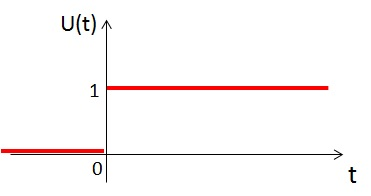
\includegraphics[width=0.9\linewidth]{images/Heaviside.jpg}
	\end{minipage}
      \end{definition}
      \begin{remarque}
        Selon l'utilisation voulue, cette fonction peut être définie
        en 0 par prolongement continu à gauche ($u(0)=0$) ou à droite
        ($u(0)=1$), ou de manière discontinue (par exemple
        $u(0)=\frac{1}{2}$ pour respecter le théorème de \Dirichlet{}
        avec les séries de \Fourier{}). On peut aussi simplement laisser
        cette fonction définie seulement sur $\R^{\star}$.
      \end{remarque}
        
      À l'aide de cette fonction, on peut définir la \emph{fonction
        porte}\footnote{On dit \emph{boxcar function} chez les saxons}, ou bien
      encore \emph{fenêtre naturelle} voire parfois \emph{fonction
        rectangle}, pour représenter le fait que l'on s'intéresse à un
      signal dans une fenêtre temporelle donnée.
        
      \begin{definition}{Fonction porte ou fenêtre naturelle}

        On note $\porteDe{a}{b}$ la fonction définie par:
        \begin{equation}
          \label{eq:porte}
          \porteDe{a}{b} \quads= t \mapsto u\de{t-a}-u\de{t-b} \quads= t\mapsto \pparMorceaux{1}{\text{si } a<t<b}{0}{\text{si } t<a \text{ ou } t>b} 
        \end{equation}

        On note $\porte$ la fonction porte unitaire définie par~:
\begin{equation}
          \label{eq:porte_unitaire}
          \Pi \quads= \porteDe{-\frac{1}{2}}{\frac{1}{2}} \quads= t\mapsto \pparMorceaux{1}{\text{si } t<\abs{1/2}}{0}{\text{si } t>\abs{1/2}} 
        \end{equation}   
      \end{definition}

      Cette fonction peut être utilisée pour approcher n'importe
      quelle autre fonction par une fonction en marches d'escalier de largeur $\Delta_\tau$ avec la forme~:
      \begin{equation}
        \label{eq:escalier}
        t\mapsto f(t)  \approx t\mapsto \sum_{k\in\Z} f\de{k\Delta_\tau}\,.\,\porteDe{0}{\Delta_\tau}\de{t-k\Delta_\tau}
      \end{equation}
      Ce type de fonction escalier est utilisé dans la définition de
      l'intégrale au sens de \grandPonte{Riemann} que l'on peut
      ré-écrire~:
      \begin{equation}
        \label{eq:integrale_escalier}
        \int\limits_{a}^{b}f(t)\,\deriv t = \lim_{\Delta\tau \to 0} \sum_{k\in\Z} \porteDe{a}{b}\de{k\Delta_\tau} \; f\de{k\Delta_\tau}\;\underbrace{\Delta_\tau}_{=\int\limits_\R\porteDe{0}{\Delta_\tau}\de{t-k\Delta_\tau}}
      \end{equation}
      où vous remarquez l'utilisation de la fonction porte $\porteDe{a}{b}$ pour annuler la fonction à intégrer en dehors des bornes fixées.

      \begin{exemple}
        Prenons une fonction en dent de scie définie par morceaux dont
        vous pouvez compléter le graphe sur la
        \figref{fig:approx_escalier} à partir de la définition
        suivante~:
        \begin{equation*}
         x : t \mapsto \ppparMorceaux
          {t+1}{\text{si } t\in\left[-1 ; 1\right[}
          {2}{\text{si }t\in\left[1 ; 2\right[}
          {0}{\text{sinon}}
          \iff x = \porteDe{-1}{1}.\p{\Id+\uniteDe{L_E}}+\porteDe{1}{2}.2\,\uniteDe{L_E}
        \end{equation*}
        comme $x$ est continue à droite, remarquez que la fonction
        porte $\porteDe{-1}{1}$ est considérée avec son prolongement à
        droite pour définir le support $\left[-1 ; 1\right[$ où la
        fonction $\Id+\uniteDe{L_E}=t\mapsto t+1$ doit être
        considérée. Une autre fonction porte est utilisée pour définir
        le support de la fonction constante
        $2\,\uniteDe{L_E}=t\mapsto 2$ et la fonction est donc laissée
        nulle ailleurs (y compris en $t=2$ puisque continue à droite).
        \begin{figure}[htbp]
          \centering
          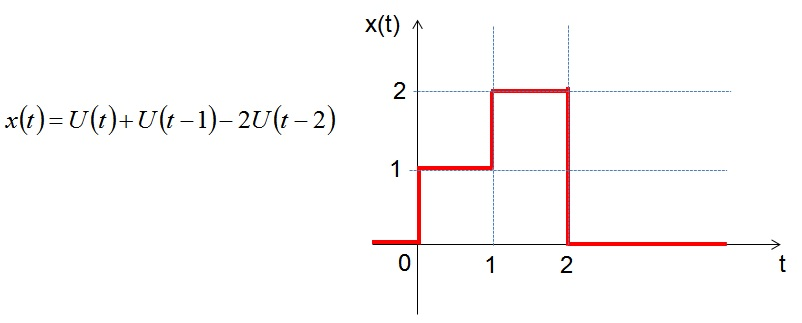
\includegraphics[scale=0.5]{images/Utilisation_Heaviside.jpg}
          \caption{Exemple d'utilisation de la fonction de Heaviside
            pour bâtir une fonction plus complexe}
          \label{fig:approx_escalier}
	\end{figure}

        Si nous approchons cette fonction en utilisant 
        \eqref{eq:escalier} avec un pas d'échantillonage
        $\Delta_\tau=1$, seuls les deux échantillons $x(0)=1$ et
        $x(1)=2$ sont non nuls et on obtient l'approximation en deux
        fonctions portes non nulles (en rouge sur
        la~\figref{fig:approx_escalier})~: ~:
        \begin{equation*}
          \forall t\in\R\quads x(t)\approx \porteDe{0}{1}\de{t}+2\porteDe{1}{2}\de{t} = \underbrace{\porte\de{t-\frac{1}{2}}}_{\text{vaut 1 autour de }0,5}+\underbrace{2\,\porte\de{t-\frac{3}{2}}}_{\text{vaut 2 autour de }1,5}
        \end{equation*}
        En remplaçant les fonctions portes par leur composition en
        fonctions de \Heaviside{}, on obtient une approximation en 3
        échelons dont l'amplitude représente le saut relatif à
        effectuer pour passer d'un escalier à un autre~:
        \begin{equation*}
          x(t) \approx \underbrace{u(t)}_{+1\text{ à }t=0} + \underbrace{u(t-1)}_{+1\text{ à }t=1} +\underbrace{ -2\,u(t)}_{-2\text{ à }t=2}
        \end{equation*}

        Cela permet d'approcher la valeur de l'intégrale de $x(t)$
        en utilisant \eqref{eq:integrale_escalier} pour avoir~:
        \begin{eqnarray*}
          &\intDt{\R}{}{x\de{t}}=\intDt{_1}{2}{x(t)}=\underbrace{\intDt{-1}{1}{t+1}}_{=2}+\underbrace{\intDt{1}{2}{2}}_{=1} = 3 \\
          \approx  &\somme{k\in\Z}{}{\porteDe{-1}{2}\p{k\Delta_\tau}x\p{k\Delta_\tau}}\Delta_\tau =  \somme{k=-1}{2}{x(k)} = \caCest{x(-1)}{=0} + \caCest{x(0)}{=1} + \caCest{x(1)}{=2} + \caCest{x(2)}{=0} = 3
        \end{eqnarray*} 
      \end{exemple}
      
      La fonction de \Heaviside{} peut servir de base pour générer
      d'autres fonctions de type causal, par intégration ou
      différenciation. Par exemple, en l'intégrant une fois, on
      obtient la \emph{fonction rampe}\footnote{appelée \emph{ramp
          function} de manière assez similaire dans les pays où l'on
        roule pourtant à gauche.} $t\mapsto t\,u(t)$. Si on l'intègre
      $n$ fois, on obtient la base des fonctions polynomiales
      causales, \cad{} nulles pour $t<0$.
	\begin{equation}\label{eq:integration_Heaviside}
          u^{(-n)}(t) = \frac{t^{n}}{!n}  u(t)	 	
	\end{equation}	où $u^{\p{n}}$ désigne la n\ieme{} dérivée et par extension $u^{\p{-n}}$ la n\ieme{} primitive qui s'annule en $0$.
        
	Le cas de la dérivation est plus complexe car elle entraîne
        l'apparition d'une discontinuité. En effet, la dérivée de la
        fonction de \Heaviside{} n'est pas définie en $0$ car non
        continue en $0$. Cet écueil ne peut se traiter qu'en utilisant
        la théorie des distributions, qui va permettre de définir
        l'impulsion de \Dirac.
	
	\subsubsection{Impulsion ou distribution de \Dirac}
	
	L'impulsion de \Dirac{} se trouve, par exemple, en
        différenciant l'échelon unitaire. On voit immédiatement
        apparaître un problème : la dérivée est nulle presque partout,
        sauf au point 0 où l'échelon présente une discontinuité et où
        sa dérivée est infinie. Au sens classique des fonctions la
        dérivée de l'échelon unité est la fonction nulle, car on ne
        peut que proposer un prolongement continu en $0$ qui vaut $0$
        pour pourvoir l'intégrer et l'intégrale devient alors nulle~!

        \begin{remarque}
          Dans l'espace des fonctions continues $\classeZero$, les
          applications (ou opérateurs puisque l'application transforme
          une fonction en une fonction) dérivée et intégrale
          sont réciproques. Ces applications sont bijectives et ont un
          noyau nul car seul la fonction nulle $\nullDe{\classeZero}$
          à pour dérivée la fonction nulle.

          En revanche dans l'espace des signaux physiques $L_E$
          considéré, pouvant donc être discontinus, on voit que au
          moins $u(t)$ et $\nullDe{L_E}$ ont pour dérivée la fonction
          nulle. Le noyau de l'application dérivée n'est plus réduit à
          $\{\nullDe{L_E}\}$ mais est au moins de dimension $1$
          puisque $\vect{u} \subset \ker{\dDtDe{}}$. Les opérateurs
          dérivée et intégrale ne sont plus réciproque.
        \end{remarque}
        
        Pourtant l'intuition physique nous pousse à penser qu'intégrer
        la dérivée d'un échelon doit redonner un échelon et qu'il
        existe bien un signal qui, donné en entrée d'un intégrateur,
        provoque un échelon en sortie. De même lorsque l'on considère
        une particule élémentaire comme une masse ponctuelle à travers
        une fonction de densité de masse, on introduit une fonction
        nulle partout sauf au point où se trouve la particule et dont
        la valeur de densité de masse est infinie, cependant sont
        l'intégrale vaut la masse de la particule. C'est pour cela que
        \Dirac{} introduit la \emph{fonction Delta} dans le
        développement de la théorie quantique des champs sans pour
        autant en donner une définition mathématique valable. Cette
        fonction apparaît aussi lorsque l'on considère la fonction de
        densité de probabilité $p(x)$ d'un événement discret tel qu'un
        jet de dé~: la densité de probabilité en dehors des nombres
        entier est nulle mais infinie pour chaque valeur de $1$ à
        $6$. Pourtant lorsque l'on veut la probabilité de tirer $1$
        sur un jet, on intègre cette densité autour de $1$ et l'on veut
        obtenir
        $\int\limits_{1-\epsilon}^{1+\epsilon}p(x) \deriv x=\frac{1}{6}$

        Il
        faudra, 30 ans plus tard, deux médailles Field et bâtir la
        théorie des \emph{Distributions} ou des \emph{fonctions
          généralisées} pour en donner une définition correcte et
        obtenir une généralisation de la notion de fonction permettant
        de dériver les fonctions non--continues en tout points~!

        Le but de cette partie n'est pas de faire une présentation
        exhaustive de la théorie des distributions, mais de donner du
        sens à cette impulsion de \Dirac, de décrire comment
        l'utiliser convenablement et de lui donner une place centrale
        dans l'études des systèmes et des signaux.

        Il est possible de donner une justification physique à
        l'impulsion de \Dirac{} par un passage à la limite, comme
        illustrée sur la figure ci-contre. On considère une fonction
        échelon avec un temps de transition finie $\tau$. En dérivant
        cette fonction, on obtient une fonction décrivant une
        impulsion brève de durée $\tau$. L'aire de cette fonction,
        associée à son intégrale sur $\R$, est égale à 1 quel que soit
        $\tau$. Par passage à la limite quand $\tau$ tends vers 0, on
        se rapproche d'une fonction nulle presque partout sauf en $0$
        où elle tend vars l'infini et dont l'intégrale vaut
        $1$. L'impulsion de \Dirac{} peut être présentée comme un
        algorithme de passage à la limite d'une impulsion, elle est
        donc décrite par \og{} son effet sous l'intégrale \fg{} et
        n'admet pas de définition classique même en tant que limite de
        fonction~:
	
        \begin{figure}[htbp]
          \begin{minipage}[l]{0.4\linewidth}
          \begin{equation}\label{Dirac_aire}
            \int_{\mathbb{R}}\delta (t)dt = 1 	
          \end{equation}
	\begin{equation}\label{Dirac_derive}
          \delta (t) = \frac{du(t)}{dt}	 	
	\end{equation}
	\end{minipage} \hfill
	\begin{minipage}[r]{0.6\linewidth}
          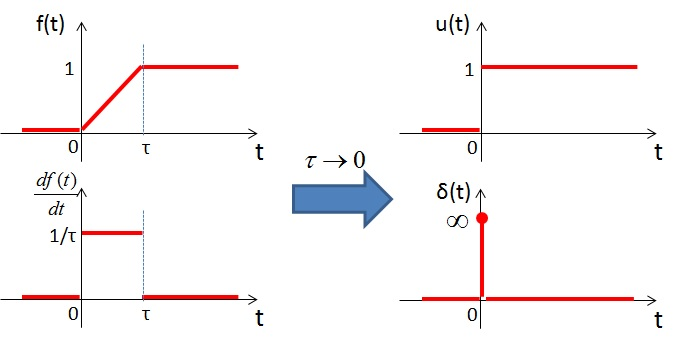
\includegraphics[scale=0.5]{images/generation_Dirac.jpg}
   	\end{minipage}
	\vspace{0.5\baselineskip}
        
        \caption{Le \Dirac{} vu par le passage à la limite d'une
          fonction continue. Attention la limite de l'impulsion
          continue lorsque $\tau\to 0$ est toujours la fonction
          nulle presque partout et non pas un \Dirac{}. Cependant son
          effet sous l'intégrale n'est pas celui de la fonction
          nulle.}
        \label{fig:dirac}
      \end{figure}
	L'impulsion de \Dirac{} est donc un objet mathématique qui
        n'est pas une fonction classique, on parle de fonction
        généralisée, qui est une dérivée non nulle de l'échelon et
        dont l'intégrale est la fonction échelon. 

        La position de cette impulsion n'est pas forcément centré en
        0. On notera $\delta_a$ la fonction généralisée dont
        l'intégrale est l'échelon centré en $a$ soit
        $u_a : t\mapsto u\p{t-a}$ et donc la fonction Delta est par
      défaut $\delta = \delta_0$. Il n'est pas rare de voir la
      fonction généralisé Delta utilisée et nommée comme une fonction
      classique, par exemple \og{} la fonction $\delta(t-a)$ \fg{} au
      lieu de la distribution $\delta_a$. Ce sont des abus de langage
      avec lesquels il faut être prudent car si certaines propriétés
      (comme ici le décalage dans le temps et donc la composition avec
      une fonction $t\mapsto t-a$ ) sont conservée par les
      distributions, d'autre ne le sont pas.
        
	% TODO ça c'est faux ! l'impulsion est infinie en 0 !
        % De manière générale, on peut écrire que la distribution ou
        %impulsion de \Dirac{} est définie par l'équation \ref{Dirac}.
	% \begin{equation}\label{Dirac}
        %   \delta (t-a) = \left \{
        %     \begin{array}{l}
        %       1~~~si~t = a \\
        %       0~~~sinon \\
        %     \end{array}
        %   \right . 	
	% \end{equation}

      %TODO pas compris pourquoi If(delta) et pas If(t0)...
	Quel peut être l'intérêt d'un tel objet mathématique, nul
        partout sauf en un point où il devient infini ? Il est certain
        qu'il ne peut être utilisé comme une fonction. Par contre, il
        peut servir à calculer une fonction indicatrice
        $I_{f}(t_0)$ pour mesurer une caractéristique d'une
        fonction f, définie en $\mathbb{R}$, autour de l'instant$t_0$.
        Comme le montre \eqref{eq:fonction_indicatrice}. La fonction $f$ est
        localement intégrable et $\delta(t)$ sert de fonction de mesure~:
	\begin{equation}\label{eq:fonction_indicatrice}
          I_{f}(t_0)=\int_{\mathbb{R}}\delta(t-t_0)f(t)dt
	\end{equation}
	
	À l'intérieur de l'intégrale, la distribution de \Dirac{}
        prend tout son sens, car elle est définie par son effet sous
        l'intégrale. Elle va permettre de mesurer la fonction f au
        point $t = t_0$. En effet, à l'intérieur de l'intégrale, en
        multipliant l'impulsion avec la fonction $f$ et en l'intégrant
        sur un intervalle infiniment court, on prélève la valeur de
        la fonction f au point $t = t_0$. On appelle cette propriété
        la propriété d'échantillonnage, donnée par
        \eqref{eq:dirac_echantillonage}. Celle-ci présente un très grand
        intérêt dans l'étude des signaux.
	
	 \begin{eqnarray}\label{eq:dirac_echantillonage}
           \int_{-\infty}^{+\infty} \delta\p{t}  f(t) \deriv t  = f(0)  \\ 
           \int_{-\infty}^{+\infty} \delta_{t_0}\, f(t) \deriv t  = f(t_0) \nonumber 
	 \end{eqnarray}
	
	Précisons-le à nouveau : l'utilisation de l'impulsion de
        \Dirac{} n'a de sens qu'à l'intérieur d'une intégrale. Ce n'est
        pas une fonction classique mais une distribution ou fonction
        généralisée. L'usage pratique montre qu'on trouve souvent
        l'impulsion de \Dirac{} utilisée à l'extérieur de toute
        intégrale, comme une fonction mathématique classique. C'est
        bien entendu une écriture abusive et potentiellement source
        d'erreur. Cependant, ce type d'écriture permet parfois une
        simplification de l'écriture des calculs, qui est toléré si
        l'impulsion de \Dirac{} est correctement employée dans une
        intégrale. Il est courant de représenter sur un graphique
        l'impulsion de \Dirac, au même titre qu'une
        fonction. Techniquement, c'est impossible car l'amplitude de
        l'impulsion de \Dirac{} devient infinie. Par convention, on la
        représente sous la forme d'un trait, terminé par une flèche,
        avec à proximité une valeur placée entre parenthèse indiquant
        l'aire du \Dirac, \cad{} l'amplitude de l'échelon obtenu par
        intégration. Cette aire est appelé \emph{poids} du \Dirac{} en
        référence à son utilisation dans les fonction densité de masse
        dont l'intégrale donne le poids de la particule.

        La figure \ref{fig:representation_dirac} illustre cette
        représentation, avec l'affichage de l'impulsion
        $2\delta_1$.
        \begin{figure}[htbp]
          \centering
          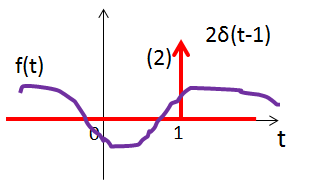
\includegraphics[scale=0.6]{images/representation_Dirac.png}
          \caption{Représentation graphique conventionnelle d'une
            impulsion de \Dirac de poids 2 et centrée en 1. Remarquez
            la notation abusive $\delta\p{t-1}$ au lieu de $\delta_1$}
          \label{fig:representation_dirac}
	\end{figure}
L'impulsion est centrée en t = 1 et son poids
        est égal à 2. Sur ce graphe, on a superposé l'impulsion de
        \Dirac{} avec le tracé d'une fonction $f$
        quelconque. L'utilisation de l'impulsion à l'intérieur de
        l'intégrale \ref{Dirac_echantillonage_2} permet d'extraire la
        valeur de f au point $t = 1$.


        Revenons au problème initial de sélection de familles
        d'excitation inchangées par l'effet d'un système LTI. On peut
        remarquer que cette propriété est aussi vérifiée avec la
        famille d'excitation impulsionnelle. L'action d'un opérateur
        proportionnel, intégrateur ou dérivée appliquée à une fonction
        de cette famille donnera une nouvelle fonction appartenant
        aussi à cette famille. De plus, on comprend intuitivement
        l'intérêt de l'impulsion de \Dirac{} pour déterminer la
        réponse temporelle d'un système à n'importe quelle
        excitation. De par sa propriété d'échantillonnage, chaque
        point d'une excitation peut être modélisée, à la limite, par
        une impulsion de \Dirac. L'excitation complète peut donc être
        modélisée comme la superposition d'un nombre infini
        d'impulsions de \Dirac. Si on sait comment le système réagit à
        une impulsion de \Dirac, la réponse à l'excitation sera la
        superposition des réponses à toutes les impulsions de \Dirac,
        puisque le système est linéaire.
	
	
	
	\section{Les différents types de réponse caractérisant les systèmes LTI}
	Maintenant que nous avons défini deux familles d'excitation
        adaptées à l'étude des systèmes LTI, nous pouvons définir
        plusieurs types de réponse qui nous aideront à analyser les
        propriétés de ces systèmes.
		
	
	\subsection{Réponse impulsionnelle}
	Elle correspond à la réponse d'un système excité par une
        impulsion de \Dirac, cette réponse est notée $h(t)$~:
        % TODODONE : faux pas son énergie, mais son poids et confusion
        % avec amplitude.
        % Même si l'amplitude de cette impulsion est infinie, son
        % énergie vaut 1.
        % Au lieu de
        % représenter cette valeur infinie, nous utiliserons la valeur
        % de 1. N'oublions pas qu'il ne s'agit pas d'une fonction mais
        % d'une distribution, qui n'a du sens qu'à l'intérieur d'une
        % intégrale.
	\begin{equation}
          h = L\b{\delta_0}
        \end{equation}
	Quel que soit le système LTI considéré, puisque l'excitation
        devient nulle pour t > 0, on retrouve le calcul de la réponse
        naturelle. L'application de l'impulsion en t=0 ne fait que
        changer les conditions initiales.
	
	\begin{equation}\label{}
          si~x(t)=\delta (t)~\rightarrow ~y_{f}(t) = y_{0}(t)	 	
	\end{equation}
	
	
	
	\vspace{1\baselineskip} La réponse impulsionnelle va nous
        fournir un moyen de calculer la réponse d'un système LTI à
        n'importe quelle excitation, en effectuant les calculs
        uniquement dans le domaine temporel. C'est ce que nous allons
        démontrer. Tout signal peut être vu comme la superposition
        d'un nombre infini de points, pouvant être modélisés par des
        impulsions de \Dirac, pondérées et décalées dans le
        temps. Comme le montre la figure
        \ref{Fig:Approx_excitation_Dirac}, une excitation quelconque
        x(t) peut être approximée par une suite de rectangles
        adjacents, de largeur $ \Delta_\tau $, que l'on peut remplacer
        par des impulsions de \Dirac{} équivalentes de même
        surface. Ainsi, elles transportent la même énergie. Si la
        largeur $ \Delta_\tau $ tend vers zéro, cette approximation
        devient de plus en plus juste. Dans l'exemple considéré, on
        suppose que x(t) = 0 pour t \textless{} 0 par souci de
        lisibilité. Le même raisonnement resterait juste avec x(t) non
        nul pour t \textless{} 0. L'excitation peut alors s'approximer
        par :
	
	
	\begin{equation*}\label{}
          \sum_{n=-\infty}^{+\infty}x(n\Delta_\tau) 	\Delta_\tau  \delta (t-n\Delta_\tau)	
	\end{equation*}
	
	\begin{figure}[htbp]
          \centering
          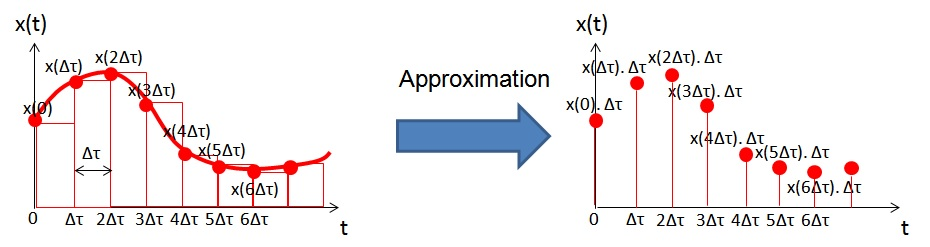
\includegraphics[scale=0.5]{images/Approx_excitation_Dirac.jpg}
          \caption{Excitation quelconque x(t) approximée par une suite
            d'impulsion de \Dirac}
          \label{Fig:Approx_excitation_Dirac}
	\end{figure}
	Supposons que cette excitation attaque l'entrée d'un système
        LTI dont la réponse impulsionnelle h(t) est connue
        (Fig. \ref{Fig:reponse_impuls_illustration}). Par souci de
        lisibilité, on suppose aussi que h(t) = 0 pour t < 0.
	\begin{figure}[htbp]
          \centering
          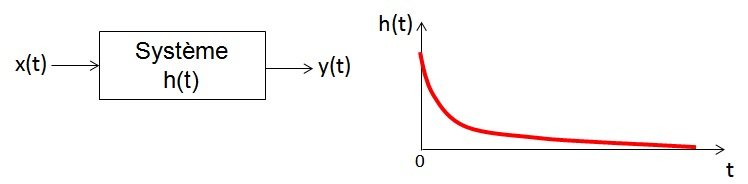
\includegraphics[scale=0.5]{images/reponse_impuls_illustration.jpg}
          \caption{Réponse impulsionnelle d'un système}
          \label{Fig:reponse_impuls_illustration}
	\end{figure}
	
	Chaque impulsion élémentaire composant x(t) et apparaissant à
        l'instant $ k \times \Delta_\tau $ contribue à la réponse en
        sortie, comme l'illustre la figure
        \ref{Fig:illustration_reponse_impuls_2}. Chacune d'entre elles
        produit une réponse égale à la réponse impulsionnelle du
        système, mais :
	
	\begin{itemize}
        \item pondérée par l'amplitude de l'excitation d'entrée à
          l'instant $ k \times \Delta_\tau $
	
        \item décalée dans le temps de $ k \times \Delta_\tau $~
	\end{itemize}
	\begin{figure}[htbp]
          \centering
          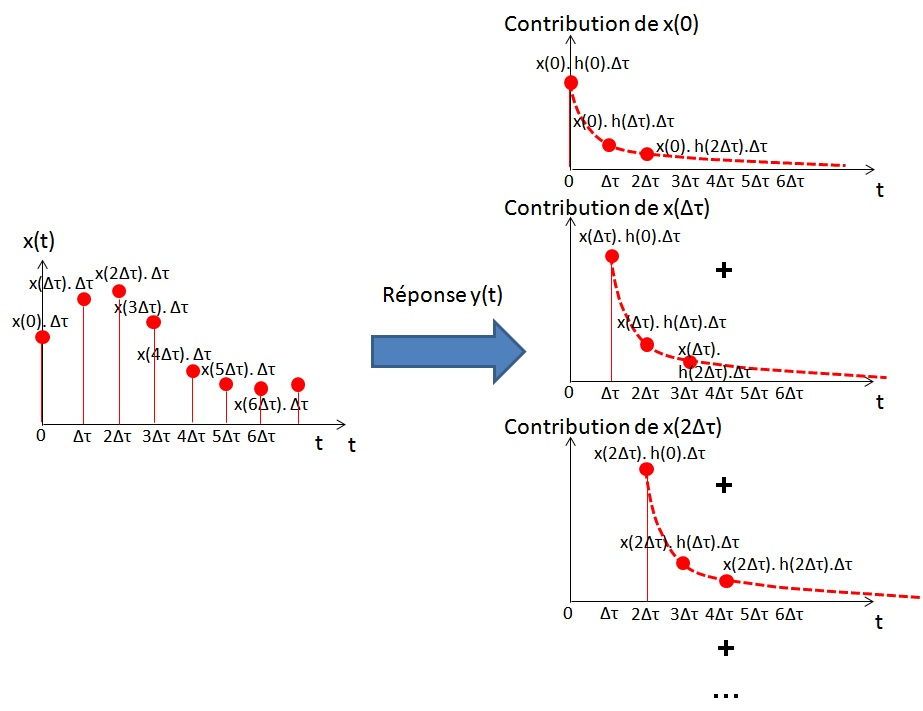
\includegraphics[scale=0.5]{images/illustration_reponse_impuls.jpg}
	\end{figure}
	\begin{figure}[htbp]
          \centering
          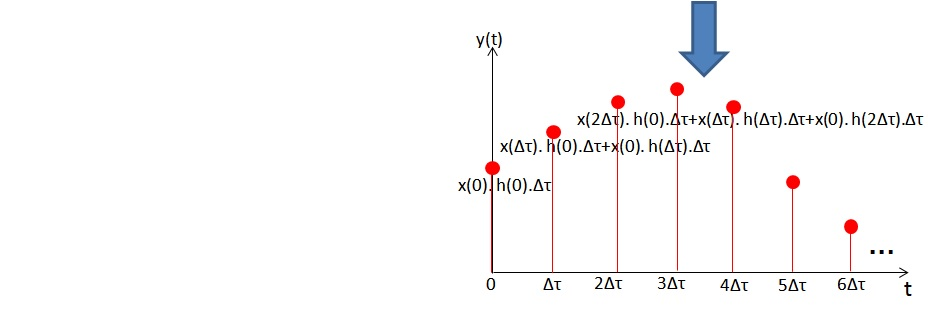
\includegraphics[scale=0.6]{images/illustration_reponse_impuls_2.jpg}
          \caption{Construction de la réponse impulsionnelle}
          \label{Fig:illustration_reponse_impuls_2}
	\end{figure}

	La réponse globale du système est obtenue en sommant
        l'ensemble des contributions de chaque impulsion élémentaire
        formant l'excitation. Elle peut alors s'approximer par :
	\begin{equation*}\label{key}
          \sum_{n=-\infty}^{+\infty} x\p{n\Delta_\tau}  \Delta_\tau  h(t-n\Delta_\tau)
	\end{equation*}
	
	En faisant tendre $ \Delta_\tau $ vers zéro, cette somme
        converge vers une intégrale donnée par la relation
        ci-dessous. Ce calcul intégral particulier, faisant intervenir
        le produit de deux fonctions dont les indices $\tau $ et
        $t-\tau $ sont balayés dans des directions opposées, porte un
        nom : le produit de convolution. Cette opération est
        symbolisée par le signe $*$.
	\begin{equation}\label{Demo_produit_convolution}
          y(t) = \lim_{\Delta_\tau \to 0} \somme{n=-\infty}{+\infty}{x\de{n\Delta_\tau}}  \;  h\de{t-n\Delta_\tau}\;\Delta_\tau = \intDt{-\infty}{+\infty}{x\de{\tau}\, h\de{t-\tau}} = x*h(t)
	\end{equation}
	
	Cette relation basée sur le produit de convolution fournit
        donc un outil de calcul de la réponse du système directement
        dans le domaine temporel. Cependant, c'est un calcul complexe,
        passant par une opération longue et fastidieuse si elle est
        effectuée à la main. Nous y reviendrons au chapitre 7, qui
        sera consacré au calcul des réponses des systèmes LTI
        directement dans le domaine temporel. Cependant, avant
        d'aborder ce point, nous allons d'abord considérer le cas
        d'une excitation exponentielle complexe pour dériver le
        concept de fonction de transfert défini dans le domaine
        fréquentiel. Nous verrons que dans ce domaine, le calcul de la
        réponse du système est beaucoup plus aisée !
	
	\subsubsection{Condition pour garantir la causalité}
	Un système est causal si sa réponse ne dépend que des états
        passés et présents. A partir de la réponse impulsionnelle, on
        peut en déduire une condition : il faut que h(t) = 0 pour t <
        0. Les systèmes causaux sont les seuls à être physiquement
        réalisables. Le calcul de la réponse d'un système causal à
        partir de sa réponse impulsionnelle peut s'écrire :
	\begin{equation}\label{}
          y(t) = \int_{0}^{+ \infty} x(\tau)  h(t-\tau)d\tau = x*h(t)
	\end{equation}
	\vspace{1\baselineskip}
	
	\subsection{Réponse indicielle}
	Elle correspond à la réponse d'un système excité par une
        fonction de Heavisde. On la note a(t).
	\begin{equation}\label{key}
          si~x(t)=u(t)~\rightarrow ~y_{f}(t)=a(t)
	\end{equation}

	\vspace{0.5\baselineskip}
	
	\textbf{\underline{Autre manière de déterminer la réponse
            impulsionnelle}}
	
	Sans démonstration, on peut affirmer que si on différencie
        l'excitation, on peut déterminer la nouvelle réponse en
        différenciant la réponse à l'excitation initiale : si
        $y(t) = L[x(t)]$ alors $\frac{dy}{dt} = L[\frac{dx}{dt}] $.
        Ainsi, puisque l'impulsion de \Dirac{} est la dérivée de
        l'échelon unitaire, si on connait la réponse indicielle, on
        peut retrouver la réponse impulsionnelle en dérivant la
        réponse indicielle.
	
	\begin{equation}\label{key}
          \delta(t)=\frac{da(t)}{dt}
	\end{equation}
	
	\vspace{0.5\baselineskip}
	
	
	\subsection{Réponse à une exponentielle complexe - Fonction de transfert}
	On considère une excitation exponentielle complexe. La réponse
        forcée a donc la même forme que l'excitation, et présente la
        même fréquence complexe. La seule inconnue est le phaseur
        $\hat{Y}$ de la réponse. Soit l'excitation
        $ x(t) = Re[\hat{X}  \expo{pt}]$ et la réponse
        $ y_{f}(t) = Re[\hat{Y}  \expo{pt}]$ pour t > 0. Si on
        reprend l'équation différentielle ordinaire générale d'un
        système LTI donnée par \ref{eq:generale_lti}, on peut
        écrire la relation suivante.
	
	\begin{equation*}\label{}
          \sum a_{i}  Re[p^{i}  \hat{Y}  \expo{pt}] = \sum b_{i}  Re[p^{j}  \hat{X}  \expo{pt}]
	\end{equation*}
	\begin{equation*}\label{}
          \sum a_{i}  Re[p^{i}  \hat{Y}] = \sum b_{i}  Re[p^{j}  \hat{X}]
	\end{equation*}
	\begin{equation*}\label{}
          \hat{Y}  \sum a_{i}  Re[p^{i}] = \hat{X}  \sum b_{i}  Re[p^{j}]
	\end{equation*}
	
	On peut donc facilement déterminer le phaseur $\hat{Y}$
        associée à la réponse, c'est-à-dire le module et le déphasage
        de la réponse.  On peut alors caractériser l'effet du système
        à une excitation exponentielle complexe quelconque sous une
        forme appelée fonction de transfert, définie comme le rapport
        entre les phaseurs de réponse et d'excitation, et défini pour
        toutes les fréquences complexes.
	\begin{equation}\label{Def_fonction_tranfert}
          H(p) = \frac{Y}{X} (p) = \frac{\hat Y}{\hat X} (p)= \frac{\sum a_{i}  Re[p^{i}]}{\sum b_{i}  Re[p^{j}]}=G\frac{\prod_{i=1}^{M} (p-p_{i})}{\prod_{j=1}^{N} (p-p_{j})}
	\end{equation}
	De manière générale, l'équation \ref{Def_fonction_tranfert} peut s'écrire comme une fraction rationnelle entre deux polynômes, où G est un terme constant. Les N racines du dénominateur sont les pôles de la fonction de transfert et les M racines du numérateur sont appelées les zéros de la fonction de transfert. Comme leur nom l'indique, ils annulent la fonction de transfert lorsque la fréquence $p=p_{j}$. Les pôles sont les mêmes que ceux identifiés dans la réponse naturelle ! Ils ont un rôle prépondérant sur la stabilité du système et la nature de la réponse. Les outils permettant d'étudier l'influence des pôles et des zéros sur la réponse d'un système sortent du cadre de ce cours et seront abordés dans les cours d'automatique.\\
	
	Avec une excitation exponentielle complexe, l'action du
        système LTI peut donc se résumer à la multiplication de
        l'excitation par la fonction de transfert.  On peut souligner
        la facilité de la méthode. Une fois la fonction de transfert
        connue à une fréquence complexe donnée, la réponse forcée à
        une exponentielle complexe de même fréquence est trouvée en
        multipliant le phaseur d'entrée par la fonction de transfert
        (\ref{Relation_Entree_Sortie_Fonction_Transfert}).
	\begin{equation}\label{Relation_Entree_Sortie_Fonction_Transfert}
          \hat{Y}(p) = H(p) \hat{X}(p)=|H(p)||X(p)|\expo{j(arg(H(p))+arg(\hat{X}(p)))}	
	\end{equation}
	
	\vspace{1\baselineskip}
	
	
	\textbf{\underline{Réponse en régime permanent :} }
	
	Dans le cas général, l'excitation est complexe. Le cas
        particulier où $\sigma$ = 0 correspond au cas d'une excitation
        dite monochromatique ou harmonique. On parlera alors de
        réponse en fréquence. Il correspond aussi au cas du régime
        permanent avec $\sigma$ < 0, c'est-à-dire que t devient
        suffisamment grand pour que l'influence du terme
        $\expo{\sigma t}$ devienne négligeable.  La réponse du système se
        trouve facilement en remplaçant la fréquence complexe p par
        $j\omega$. En considérant une excitation cosinusoïdale
        d'amplitude égale à X et de phase $\Phi_{x}$, la réponse du
        système est donnée par la relation suivante.
	
	\begin{equation}\label{calcul_reponse_fonction_transfert}
          y(t) = Re[|H(\omega)|X e^{j(\omega t+arg(H(p))+\Phi_{x})}] =|H(\omega)|X cos(\omega t+arg(H(p))+\Phi_{x})
	\end{equation}
	
	La réponse est une grandeur complexe. Le module de la réponse
        en fréquence est le gain en amplitude de la fonction de
        transfert du système ou du filtre. Le déphasage du signal en
        sortie du filtre par rapport au signal d'entrée est l'argument
        de la fonction de transfert. Le module et la phase sont des
        fonctions de la pulsation $\omega$.
	
	
	\subsubsection{Exemple}
	
	\begin{minipage}[l]{0.7\linewidth}
          On reprend l'exemple du circuit RC abordé dans la partie
          IV.4. On considère toujours que le condensateur est chargé
          initialement en t = 0, avec une tension à ses bornes notée
          $U_C0$. Le circuit est excité par un signal délivrant une
          excitation exponentielle complexe $U_{E}(t)=Xe^{pt}$ avec t
          > 0 et X l'amplitude complexe. La réponse du circuit
          correspond à la tension mesurée aux bornes de la résistance
          R ou tension de sortie. Déterminez la fonction de transfert
          de ce circuit. Indiquez quels sont les pôles et les
          zéros. Quelle est la réponse à un signal cosinuoïdal,
          d'amplitude unitaire et de phase nulle ?
	\end{minipage} \hfill
	\begin{minipage}[r]{0.4\linewidth}
          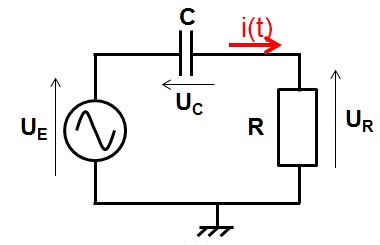
\includegraphics[scale=0.5]{images/circuit_RC_reponse_forcee.jpg}
	\end{minipage}
	\vspace{0.5\baselineskip}

	La réponse du circuit $U_{R}$ est la superposition de la
        réponse naturelle $U_{R0}$ et de la réponse forcée
        $U_{Rf}$. La réponse naturelle est liée à la présence d'une
        condition initiale : ici, le stockage d'une charge dans le
        condensateur à t=0. Sans charge initialement stockée, la
        réponse naturelle aurait été nulle. Nous avions établi la
        réponse naturelle de ce circuit en terme de courant. Nous
        pouvons aisément l'adapter pour la donner en terme de tension
        de sortie.
	\begin{equation*}\label{}
          U_{R0}(t)=Ri_{0}(t)=U_{C0}\expo{-\frac{t}{RC}}~,~~t>0
	\end{equation*}

        La réponse forcée est provoquée par l'excitation du circuit en
        t > 0, indépendamment de la présence d'une condition
        initiale. Commençons par établir une équation différentielle
        reliant la tension de sortie $U_{Rf}$ et l'excitation
        $U_{E}(t)$. On utilise la loi des mailles. Après une
        dérivation, on obtient l'équation
        \ref{equa_diff_reponse_forcee_RC}.
	\begin{equation*}\label{}
          U_{E}(t)=U_{C}(t)+U_{R}(t) ~ \Rightarrow ~ U_{E}(t)=\frac{1}{C}\int i(t) \deriv t+U_{R}(t)~ \Rightarrow ~U_{E}(t)=\frac{1}{RC}\int U_{R}(t) \deriv t+U_{R}(t)
	\end{equation*} 
	\begin{equation}\label{equa_diff_reponse_forcee_RC}
          \frac{dU_{E}}{dt}=\frac{U_{R}}{RC}+\frac{dU_{R}}{dt}
	\end{equation}

	L'excitation étant de type exponentielle complexe et le
        circuit linéaire, la réponse est aussi de type exponentielle
        complexe. Elle s'écrit : $U_{Rf}(t)=Y\expo{pt}$. Replaçons les
        termes $U_{E}$ et $U_{R}$ par leurs expressions respectives
        dans \ref{equa_diff_reponse_forcee_RC} et exprimons le rapport
        entre ces deux grandeurs pour obtenir la fonction de transfert
        H(p) de ce circuit (équation \ref{TF_RC_forcee}).
	\begin{equation*}
          pX\expo{pt}=\frac{1}{RC} Y\expo{pt}+pY\expo{pt} ~\Rightarrow~pU_{E}(t)=\frac{1}{RC}U_{Rf}(t)+pU_{Rf}(t)
	\end{equation*}
	\begin{equation}\label{TF_RC_forcee}
          H(p)=\frac{U_{Rf}}{U_{E}}(p)=\frac{p}{p+\frac{1}{RC}}=\frac{p}{p+\omega_{0}}~,~\omega_{0}=\frac{1}{RC}
	\end{equation}

	La fonction de transfert du système présente un zéro nul et un
        seul pôle $p_{0}$, qui est exactement le même que celui
        identifié dans l'analyse de la réponse naturelle. Ce n'est pas
        une surprise car les pôles agissent sur la stabilité, qui est
        une caractéristique intrinsèque du système indépendante de
        l'excitation. Le pôle étant purement réel et négatif, on peut
        conclure que le système sera stable.
		
	Calculons maintenant la réponse forcée à un signal
        cosinusoïdale, en utilisant
        \ref{calcul_reponse_fonction_transfert}. Le système n'agit que
        sur l'amplitude et la phase de l'excitation. Il est donc
        intéressant d'exprimer la fonction de transfert sous la forme
        de son module et son déphasage. En considérant $p=j\omega$,
        celles-ci sont :
	\begin{equation*}
          |H(\omega)|=\frac{\omega}{\sqrt{\omega^{2}+\omega_{0}^{2}}}~~~et~~Arg(H(\omega))=\frac{\pi}{2}-atan(\frac{\omega}{\omega_{0}})
	\end{equation*}
	\begin{equation*}
          \Rightarrow~U_{Rf}(t)=|H(\omega)|cos(\omega t+Arg(H(\omega)))
	\end{equation*}
	La réponse étant la superposition des réponses naturelles et
        forcées, celle-ci s'écrit :
	\begin{equation*}
          \Rightarrow~U_{R}(t)=U_{Rf}(t)+U_{R0}(t)=|H(\omega)|cos(\omega t+Arg(H(\omega)))+U_{C0}\expo{-\frac{t}{RC}}
	\end{equation*}
	
	\vspace{1\baselineskip}

	\subsection{Calcul de la réponse d'un système dans le domaine
          temporel ou fréquentiel ?}
	
	Nous venons de décrire deux manières de calculer l'effet d'un
        système LTI, selon que l'on considère une excitation
        impulsionnelle ou exponentielle complexe. Dans le premier cas,
        la réponse est déterminée directement dans le domaine temporel
        à l'aide de l'équation \ref{Demo_produit_convolution} et de la
        réponse impulsionnelle, à l'aide d'un produit de
        convolution. Dans le second cas, la réponse est déterminée
        dans le domaine fréquentiel à l'aide de l'équation
        \ref{calcul_reponse_fonction_transfert} et de la fonction de
        transfert.  Bien qu'il semble plus naturel de faire le calcul
        de la réponse directement dans le domaine temporel, nous avons
        montré que le calcul dans le domaine fréquentiel était
        beaucoup plus évident. Il se résume à une simple
        multiplication de l'excitation par la fonction de transfert.
        Cependant, comme il s'agit du même système, il y a
        nécessairement un lien entre la réponse impulsionnelle et la
        fonction de transfert. C'est ce que nous verrons dans les
        prochains chapitres, où nous aborderons les questions de
        transformée de Laplace, puis de Fourier. Nous allons ainsi
        mettre en évidence des transformations mathématiques,
        permettant le passage d'une fonction du domaine temporel au
        domaine fréquentiel, et inversement.
	
	\vspace{1\baselineskip}

	
	
	\section{Exercices}
	
	\subsubsection{Exercice 1} 
	Soient les systèmes dont le comportement temporel est défini
        par les équations suivantes. Indiquez si ces systèmes sont
        linéaires, à temps invariant et causaux ?
	
	a. $y(t) = x(t)+4\frac{dy}{dt}$
	
	b. $y(t) = 2x(t)+2$
	
	c. $y(t)=\expo{-t}x(t-2)^{2}$
	
	d. $y(t)=\frac{dx}{dt}+x(t+2)$
	
	\vspace{1\baselineskip}
	
	\subsubsection{Exercice 2} 
	1. On trace les réponses de deux systèmes LTI ((a) et
        (b)). Proposez une expression mathématique décrivant ces
        réponses.
	\begin{figure}[htbp]
          \centering 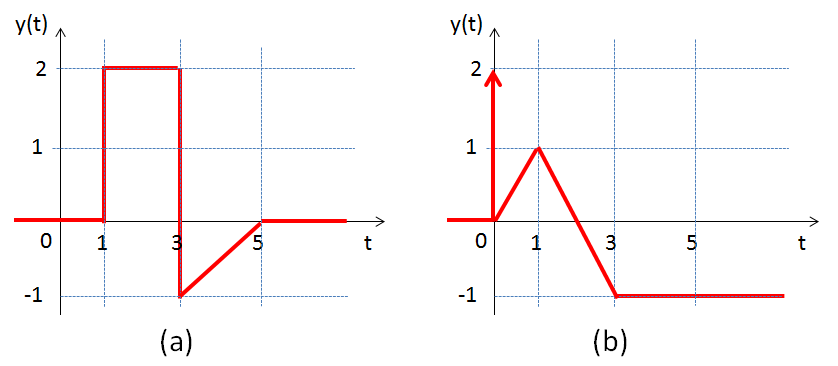
\includegraphics[scale=0.5]{images/Exo_2_2.jpg}
	\end{figure}

	
	2. Réécrivez sous la forme d'une fonction à valeurs réelles
        les fonctions suivantes et esquissez leur forme temporelle
        (pour t >0) :
	
	a. $x(t) = (1+j)\expo{j 10t}$
	
	b. $y(t) = \expo{(-2+j)t} u(t-2)$
	
	c. $z(t) = \expo{(-1+2j)t}+\expo{(-1-2j)t}$
	
	\vspace{1\baselineskip}
	
	
	
	\subsubsection{Exercice 3}
	
	On dispose de la réponse indicielle d'un système linéaire, qui est esquissée ci-dessous. Elle a une forme exponentielle croissante.\\
	
	\begin{figure}[htbp]
          \centering 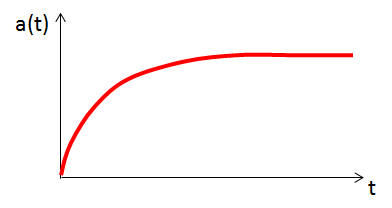
\includegraphics[scale=0.5]{images/Exo_2_3.png}
	\end{figure}
	
	Esquissez les réponses de ce système dans les cas suivants :\\
	
	a. l'excitation $e(t)=u(t)-u(t-1)$\\
	
	b. l'excitation $e(t)=t(u(t)-u(t-2))$\\
	
	c. l'excitation est la dérivée de celle utilisée pour obtenir la réponse indicielle.\\
	
	\subsubsection{Exercice 4}
	
	On excite un système linéaire à l'aide du signal suivant : $e(t)=\expo{j2\pi t}$. La réponse obtenue, notée y(t), est égale à $y(t)=\frac{1}{2}\expo{j(2\pi t+\frac{\pi}{3})}$.\\
	
	a. Réécrire la réponse sous la forme $y(t)=Acos(\omega t + \phi)$ et $y(t)=Bcos(\omega t)+Csin(\omega t)$, en précisant les valeurs de A, B, C et $\phi$.\\
	
	b. Donnez l'expression de la réponse du système lorsqu'il est
        excité par le signal ci-dessous.
	
	\begin{figure}[htbp]
          \centering 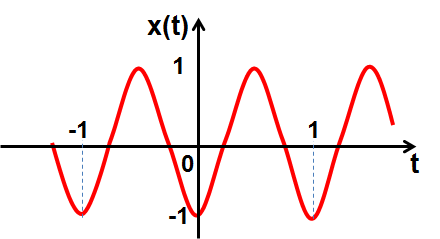
\includegraphics[scale=0.5]{images/Exo_2_4.png}
	\end{figure}
	
	c. Calculez la réponse du système à l'excitation suivante : $x(t)=\frac{3\sqrt{3}}{2}cos(2\pi t)+\frac{1}{2}sin(2\pi t)$.\\
	
	
	
	\subsubsection{Exercice 5 - Réponse indicielle d'un circuit
          RC}
	
	On reprend le circuit RC dont on a étudié la réponse dans la
        partie VI.3. On considère deux cas : celui où le condensateur
        est déchargé initialement, puis celui où il est chargé.
	
	a. Calculez la réponse naturelle du circuit lorsque le
        condensateur est initialement chargé.
	
	b. En déduire la réponse impulsionnelle du circuit.
	
	c. Calculez la réponse lorsque le circuit est soumis à un
        échelon de \Heaviside{} d'amplitude E, dans les deux cas (charge
        initiale absente ou présente).
	
	d. En déduire la réponse indicielle du circuit.
	
	\vspace{1\baselineskip}
	

	
	\subsubsection{Exercice 6}
	
	On considère les deux circuits électriques ci-dessous. Pour le
        circuit (a), la tension initiale (t=0) aux bornes du
        condensateur C est notée $U_{C0}$. Pour le circuit (b), un
        courant noté $I_L0$ traverse la bobine L. La sortie de ces
        deux circuits est la tension $U_{S}$.
	
	\begin{figure}[htbp]
          \centering 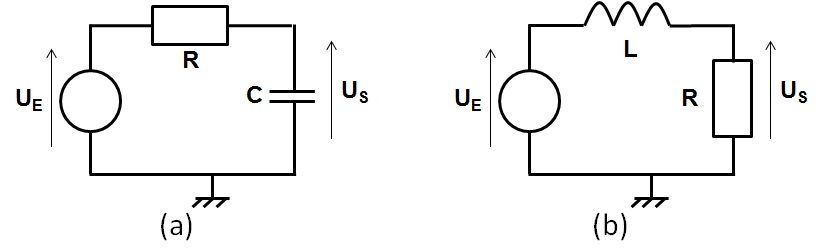
\includegraphics[scale=0.5]{images/Exo_2_4.jpg}
	\end{figure}
	
	a. Déterminez les fréquences et les réponses naturelles de ces
        deux circuits. Quels sont les ordres de ces deux systèmes ?
	
	b. On excite ces deux systèmes à l'aide d'un échelon de
        \Heaviside{} d'amplitude notée E. Déterminez la réponse
        indicielle de ces deux circuits.
	
	c. Déterminez les fonctions de transfert de ces deux circuits.
	
	\vspace{1\baselineskip}
	
	\subsubsection{Exercice 7 - Fonction de transfert d'un circuit
          résonant}
	
	On reprend le circuit RLC présenté dans la partie
        IV.4. Celui-ci est excité par un générateur de courant I,
        comme le montre la figure ci-dessous. On s'intéresse à la
        tension U aux bornes de ce circuit. On considère que la
        résistance R est grande et $R>>\sqrt{\frac{L}{C}}$.
 	 	
 	\begin{figure}[htbp]
          \centering 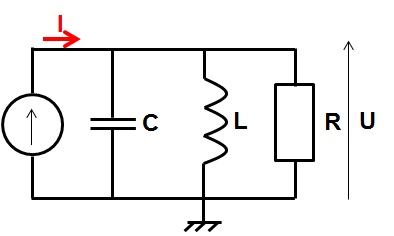
\includegraphics[scale=0.5]{images/Exo_2_5.jpg}
 	\end{figure}
 
 	a. Déterminez la fonction de transfert de ce circuit. La mettre sous la forme $\frac{Gp}{p^2+2\alpha p+\omega_{0}^{2}}$.\\
 	
 	b. Précisez l'unité de la fonction de transfert. \\
 	
 	c. Ce circuit est-il stable ?\\
 	
 	d. On considère maintenant que le terme $\alpha$ est négligeable et une excitation cosinusoïdale du circuit. Y a t-il une fréquence particulière où la réponse présente un maximum ? Si oui, laquelle ? \\
 	
 	e. Donnez l'expression de la réponse temporelle du circuit en régime permanent.\\
	
	\vspace{1\baselineskip}
	
	\subsubsection{Exercice 8}
	
	On considère le système dont le fonctionnement est décrit par
        le schéma-bloc ci-dessous. Celui-ci transforme un signal
        d'entrée e(t) et délivre en sortie un signal s(t).
	
	\begin{figure}[htbp]
          \centering 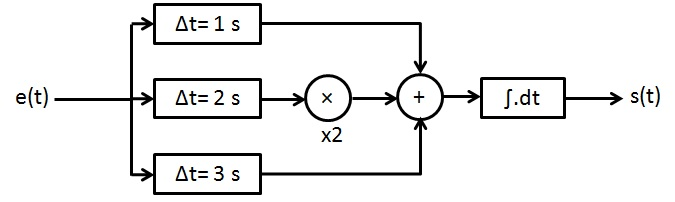
\includegraphics[scale=0.5]{images/Exo_2_6.jpg}
	\end{figure}
	
	a. Le système est-il linéaire, à temps invariant, causal ?
	
	b. Ecrire l'équation différentielle générale de ce système.
	
	c. Déterminez l'expression de la réponse impulsionnelle h(t)
        du système. Esquissez l'allure temporelle de la réponse
        impulsionnelle.
	
	d. Déterminez l'expression de la fonction de transfert H(p) du
        système. Précisez les pôles de la fonction de transfert. Que
        concluez-vous sur sa stabilité ?
	

	



        %%% Pour compiler avec emacs Local Variables: mode: latex
        %%% TeX-master: "main" End:
